\documentclass[article]{IEEEtran}
\usepackage[utf8]{inputenc}
\usepackage[pdftex]{graphicx}
\graphicspath{./}

\begin{document}

\title{Jogo do Choque}

\author{Danilo Souza, Hugo Santos, Welton Ara\'ujo

%\thanks{Engenharia da Computa\c{c}\~ao, Universidade Federal do Par\'a, Bel\'em-PA, Brasil}
Emails: \{dhcsouza, hugoleonardoeng07, weltonmaxx007\}@gmail.com\\
Matr\'iculas: 10080000801, 10080000701, 10080000501}

\maketitle

\begin{abstract}
There is a lot of possibilities to do with microcontrollers because they are very flexible. This project implements a multiplayer shock game for 2 until 4 players. The code was made on machine language, in other words Assembly with specifics instructions for the PIC16F628A. This PIC has several limitations, but could perfectly attend the game requirements in this case.
\end{abstract}

\begin{IEEEkeywords}
microcontroller, PIC16F628, game, shock, multiplayer
\end{IEEEkeywords}

\IEEEpeerreviewmaketitle


\section{Introduçao}
O PIC16F628A faz parte da família PIC de microcontroladores da Microchip Technology, composta também por diversos outros modelos, como o PIC16F627, PIC16F648, que diferem somente na	capacidade de memória flash disponível para armazenamento de programas, que para o PIC16F628A é de 2048 palavras de 32 bits (8KB)

A família PIC é amplamente utilizada hoje em dia devido à sua facilidade de programação e uma grande documentação disponível, suas aplicações podem variar desde simples protótipos até automação industrial, sua flexibilidade garante sua utilização em praticamente qualquer indústria.

A partir disto, o projeto abordado neste artigo aproveitou a possibilidade de implementar um jogo eletrizante para vários jogadores no PIC16F628A por ser um um dispositivo simples, de baixíssimo custo, porém com uma linguagem padrão Assembly.

\section{Descrição do Projeto}
O projeto baseia-se em um jogo, onde o objetivo é não levar choque, o brinquedo possui 4 controles com um botão cada e uma luz no meio, usada para indicar a hora em que os jogadores devem apertar os botões, o último que ficar por último leva um choque. As Figuras \ref{fig:jogochoque1} e \ref{fig:jogochoque2} mostram como é o dispositivo do jogo.

	\begin{figure}	
		\centering
		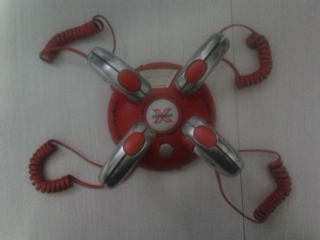
\includegraphics[width=8.5cm]{./dispositivo1.png}
		\caption{Ilustração do jogo vista de cima}
 		\label{fig:jogochoque1}
	\end{figure}

	\begin{figure}	
		\centering
		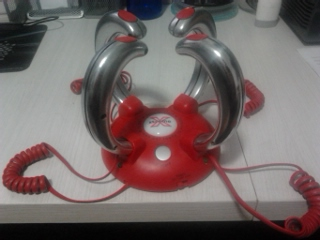
\includegraphics[width=8.5cm]{./dispositivo2.png}
		\caption{Ilustração do jogo vista de lado}
 		\label{fig:jogochoque2}
	\end{figure}

Ao começo do jogo um LED fica aceso, a rodada termina quando o LED apaga e o perdedor  leva um choque que é descarregado no próprio controle, onde há componentes metálicos. Caso algum jogador aperte o botão antes do tempo, este também levará choque como punição.

Para o projeto foram usados 4 botões, um para cada jogador, 2 LED's para cada botão de jogador, sendo um para indicar que aquele jogador está participando do jogo e outro para indicar que aquele jogador levou um choque, um outro botão para representar o \textit{start}, mais um botão para escolher o número de jogadores, sendo no mínimo 2 e no máximo 4 e um outro LED para indicar o começo de uma rodada. 
 
\section{Funcionamento do Programa}
O algoritmo de funcionamento do programa funciona com o auxílio das variáveis da Tabela \ref{tab:variaveis} onde também são descritas suas funções de controle. A Tabela \ref{tab:bits} contém os pinos do PIC utilizados como saídas e entradas juntamente com suas funções. A Figura \ref{fig:fluxograma} mostra o fluxograma das rotinas  mais determinantes do código.

\begin{figure}	
		\centering
		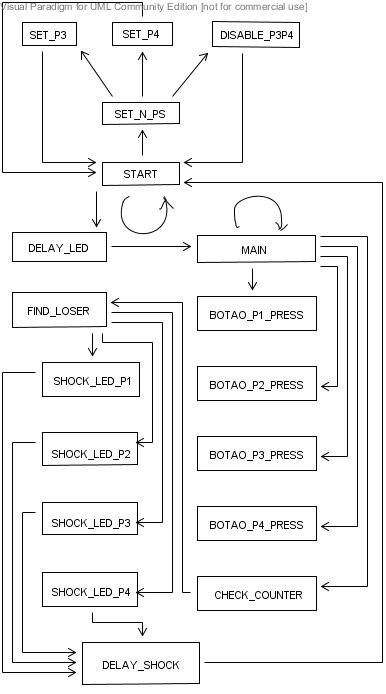
\includegraphics[width=8.5cm]{./fluxograma.jpg}
		\caption{Fluxograma de rotinas}
 		\label{fig:fluxograma}
\end{figure}

Inicialmente, no \textit{loop} da rotina \textit{START}, o programa tem somente dois botões como entrada, \textit{BOTAO\_START} para iniciar e \textit{BOTAO\_N\_PS} para definir o número de jogadores da partida. Na seleção do número de jogadores, os bits \textit{BOT,2} e \textit{BOT,3} são setados ou limpados enquanto que a variável \textit{COUNTER} inicia como 0, 1 ou 2 para 4, 3 ou 2 jogadores, respectivamente. Isso se deve porque, logo que o contador atinge um valor igual a 3, o perdedor deve levar um choque.

Ao pressionar o botão de selecionar o número de jogadores, a rotina \textit{SET\_N\_PS} é chamada onde os bits \textit{ENABLED\_LED\_P3} e \textit{ENABLED\_LED\_P4} são lidos, caso tenham valor lógico alto, significa que os jogadores 3 e 4, respectivamente, estão habilitados e a rotina \textit{DISABLE\_P3P4} é chamada para desabilitá-los. Caso somente 2 estiverem habilitados, o jogador 3 é habilitado pela rotina \textit{SET\_P3} onde bit \textit{ENABLED\_LED\_P3} é setado para alto. Em último caso, se houverem 3 habilitados, a rotina \textit{SET\_P4} é chamada para setar como 1 o bit \textit{ENABLED\_LED\_P4}.

No começo de uma partida, o programa passa a operar no delay da rotina \textit{DELAY\_LED}. Sua função é manter \textit{START\_LED} setado até o momento de limpá-lo e os botões do jogo serem apertados, porém também checa constantemente, na sua ``subrotina'' \textit{DELAY2\_LED}, as entradas do botões do jogo para punir com um choque, através das rotinas \textit{SHOCK\_P1}, \textit{SHOCK\_P2}, \textit{SHOCK\_P3} e \textit{SHOCK\_P4}, o jogador que apertar o botão antes da hora certa e, em seguida. esperar o início de uma nova partida.

Quando o \textit{START\_LED} apagar, o programa estará rodando no loop da rotina \textit{MAIN}, definido como momento de decisão, onde os botões do jogo são novamente checados. Caso algum seja apertado, alguma das rotinas \textit{BOTAO\_P1\_PRESS}, \textit{BOTAO\_P2\_PRESS}, \textit{BOTAO\_P3\_PRESS} ou \textit{BOTAO\_P4\_PRESS} são chamadas para, além de incrementar 1 no valor de \textit{COUNTER}, setar o bit \textit{BOT,0} , \textit{BOT,1} , \textit{BOT,2} ou \textit{BOT,3} , respectivamente para cada jogador.

Durante o momento de decisão, os botões \textit{BOTAO\_P1}, \textit{BOTAO\_P2}, \textit{BOTAO\_P3} e \textit{BOTAO\_P4} passam a ser funcionais. No entanto, realmente funcionarão somente o botão daqueles jogadores que foram habilitados. Por exemplo, caso sejam somente dois oponentes, os botões \textit{BOTAO\_P3} e \textit{BOTAO\_P4} ainda funcionam como entrada, porém os seus estados de pressionado ou não já foram setados para o estado pressionado durante a selecão do número de jogadores, isto é, neste caso, \textit{BOT,2} e \textit{BOT,3} estão setados como 1 fazendo-os indeferentes neste momento.

Ademais, a variável \textit{COUNTER} já foi incrementada em 1 para cada jogador desabilitado ou vice-versa para cada jogador é reabilitado. Os valores de \textit{BOT} e \textit{COUNTER} são armazenados em \textit{LAST\_COUNTER} e \textit{LAST\_BOT}. 

Ainda dentro do loop da \textit{MAIN}, existe uma rotina chamada \textit{CHECK\_COUNTER}. Nesta rotina, a variável \textit{COUNTER} é checada à procura de um valor igual a 3 para fazer a chamada da rotina \textit{FIND\_LOSER}.

A rotina \textit{FIND\_LOSER} procura pelo primeiro 0 entre os bits de \textit{BOT,0} , \textit{BOT,1} , \textit{BOT,2} e \textit{BOT,3} , nesta ordem, para setar algum dos bits de \textit{SHOCK\_LED\_P1}, {SHOCK\_LED\_P2}, {SHOCK\_LED\_P3} e {SHOCK\_LED\_P4} como 1 simbolizando o choque, respectivamente para o jogadores 1, 2, 3 e 4.

Em sequência, chama a rotina \textit{DELAY\_SHOCK} que limita a duração do choque, limpa os bits \textit{SHOCK\_LED\_P1}, \textit{SHOCK\_LED\_P2}, \textit{SHOCK\_LED\_P3} e \textit{SHOCK\_LED\_P4}, carrega os valores de \textit{LAST\_COUNTER} e \textit{LAST\_BOT} em \textit{COUNTER} e \textit{BOT}, respectivamente, para recomeçar o jogo com a última configuração de jogadores.

\begin{table}
  \centering
  \caption{Variáveis de controle}
  \vspace{0.5cm}
  \label{tab:variaveis}
  \begin{tabular}{|p{2cm}|p{1cm}|p{3.3cm}|} \hline
    Variáveis 		& Endereco & Descrição 						\\ \hline
    COUNTER		& 0x20	   & Contador do número de botões apertados antes
				     de detectar quem perdeu a partida			\\ \hline
    LAST\_COUNTER	& 0x21	   & \textit{Backup} da configuração de CONT		\\ \hline
    BOT			& 0x22	   & Campo de 8 bits responsável por memorizar
				    		 o estado de apertado ou não durante o 
				     		 momento de decisão da partida			\\ \hline
    LAST\_BOT	& 0x23	   & \textit{Backup} da configuração de BOT 		\\ \hline  
    COUNT1		& 0x24	   & Contador 1 para o delay de duração do choque	\\ \hline
    COUNT2		& 0x25	   & Contador 2 para o delay de duração do choque	\\ \hline
    COUNT3		& 0x26	   & Contador 3 para o delay de duração do choque	\\ \hline
  \end{tabular}
\end{table}

\begin{table}
  \centering
  \caption{Bits de controle}
  \vspace{0.5cm}
  \label{tab:bits}
  \begin{tabular}{|p{2.3cm}|p{1cm}|p{4cm}|}\hline
    Bits 		& Pino		& Descrição						\\ \hline
    BOTAO\_P1		& PORTA,0	& Botão para mudar o estado do jogador 1 durante
					  o momento de decisão da partida			\\ \hline
    BOTAO\_P2		& PORTA,1	& Botão para mudar o estado do jogador 2 durante
					  o momento de decisão da partida			\\ \hline
    BOTAO\_P3		& PORTA,2	& Botão para mudar o estado
				   	do jogador 3 durante
					o momento de decisão da partida			\\ \hline
    BOTAO\_P4		& PORTA,3	& Botão para mudar o estado do jogador 4 durante o momento de decisão da partida			\\ \hline
    BOTAO\_START	& PORTA,4	& Botão para iniciar a partida				\\ \hline
    BOTAO\_N\_PS	& PORTA,5	& Botão para escolher o número de jogadores da partida	\\ \hline
    SHOCK\_LED\_P1	& PORTB,0	& LED que simboliza o sinal de choque no jogador 1	\\ \hline
    SHOCK\_LED\_P2	& PORTB,1	& LED que simboliza o sinal de choque no jogador 2	\\ \hline
    SHOCK\_LED\_P3	& PORTB,2	& LED que simboliza o sinal de choque no jogador 3	\\ \hline
    SHOCK\_LED\_P4	& PORTB,3	& LED que simboliza o sinal de choque no jogador 4	\\ \hline
    ENABLED\_LED\_P3	& PORTB,4	& LED indicador de participação do jogador 3 na partida	\\ \hline
    ENABLED\_LED\_P4	& PORTB,5	& LED indicador de participação do jogador 4 na partida	\\ \hline
    START\_LED		& PORTB,6	& LED que sinaliza o início do momento de decisão	\\ \hline
  \end{tabular}
\end{table}

\section{Simulaçao}
A simulaçao foi feita no \textit{software} Proteus, o circuito lá montado buscava somente simular o funcionamento do projeto da forma mais simples e clara possivel. Portanto, não foram adotados circuitos de proteção para o funcionamento idêntico ao do projeto de \textit{hardware}. 

A Figura \ref{fig:4jogadores} mostra o momento em que o número de jogadores podem ser selecionados. Os LED's verdes acesos indicam que aquele jogador está participando da partida. Por conseguinte, ao mudar o número de jogadores, os dois LED's da direita poderiam ser acesos ou apagados.

A Figura \ref{fig:delaystart} mostra o LED vermelho aceso. Este LED fica aceso por alguns poucos segundos e apaga para os jogadores apertarem o botão. Se apertar antes da hora, acontece o processo da Figura \ref{fig:choqueP2}.

A Figura \ref{fig:choqueP2} mostra o LED amarelo aceso. Este LED simboliza a saída para o circuito de dar o choque. No caso desta figura, o perdedor foi o jogador 2. Por conta disso, o LED acendeu.

	\begin{figure}	
		\centering
		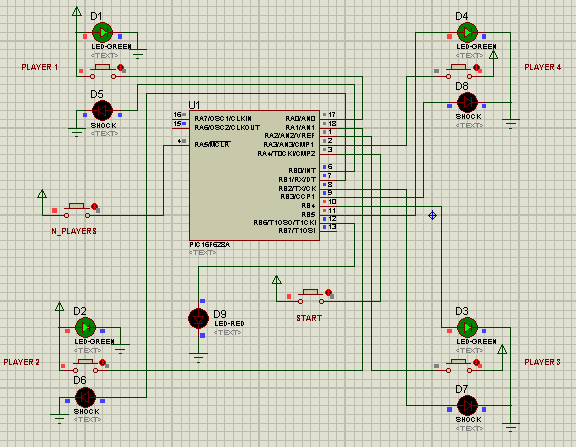
\includegraphics[width=8.5cm]{./4jogadores.png}
		\caption{Ilustração da simulaçao configurando para 4 jogadores e aguardando o inicio da partida}
 		\label{fig:4jogadores}
	\end{figure}
	
	\begin{figure}	
		\centering
		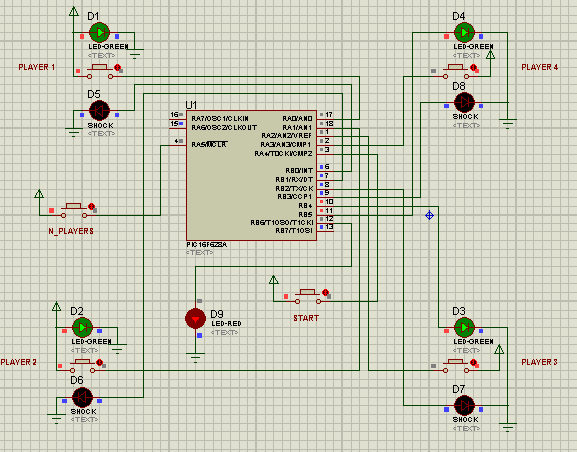
\includegraphics[width=8.5cm]{./delaystart.png}
		\caption{Ilustração da simulaçao que os jogadores esperam o LED vermelho apagar para apertar o botão}
 		\label{fig:delaystart}
	\end{figure}

	\begin{figure}	
		\centering
		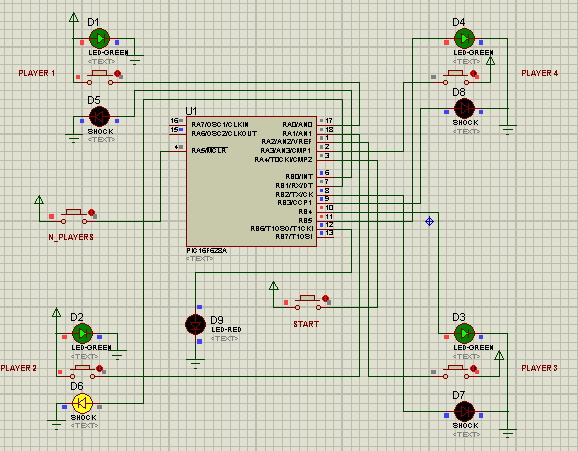
\includegraphics[width=8.5cm]{./choqueP2.png}
		\caption{Ilustração da simulaçao que mostra o jogador 2 levando um choque representado pelo LED amarelo aceso}
 		\label{fig:choqueP2}
	\end{figure}

\section{Diferenças do Jogo Original}
No jogo original, há algumas implementaçoes mais interativas com os usuários enquanto a partida ocorre e serão descritas a seguir.

Existe um \textit{buzzer} que toca uma melodia característica para o jogo. Diferentemente do LED que acende e apaga para sinalizar o momento de decisão, há um LED vermelho que fica piscando para indicar que foi dado início à partida e mais um outro com a mesma função do \textit{START\_LED}, porém ele é da cor verde e acende no momento de decisão.

\section{Conclusão}
A idéia do projeto da uma idéia muito grande de simplicidade para implementaçao, isto não deixa de ser verdade pensando em implementar em linguagens de níveis mais alto, como C e Java. Em Assembly, os conhecimentos do grupo em linguagem de máquina foram essenciais para a conclusão do projeto e o tempo de conclusão foi significativamente aumentado comparado a uma linguagem de alto nível.

O projeto funciona de uma forma mais básica em relação ao jogo original, porém realiza perfeitamente a mesma proposta de jogo para múltiplos jogadores até mesmo com memória para iniciar uma nova partida com as mesmas configuraçoes da partida anterior, tornando mais confortável a jogabilidade.  

\begin{thebibliography}{eu}
\bibitem{multicores:whitepaper}
http://pt.scribd.com/doc/20282565/Apostila-Microcontrolador-PIC-16F628
\end{thebibliography}


\end{document}